\chapter{Scheduling}

\section{Thread scheduler}

The scheduler in Zeke is conceptually object oriented and all scheduling
entities, CPUs as well as scheduling policies are implemented as objects in the
scheduling system. Each CPU can be technically populated with a different set of
scheduling policies that are then only executable on that particular CPU, see
figure \ref{figure:objscheds}.

\begin{figure}
  \center
  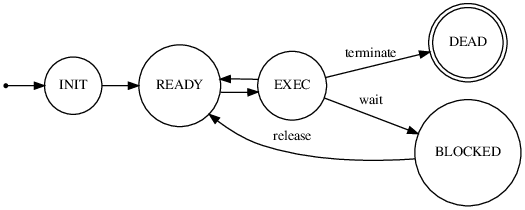
\includegraphics[width=10cm]{gfx/thread-states}
  \caption{Thread states in the scheduler.}
  \label{figure:threadstates}
\end{figure}

\begin{figure}
  \center
  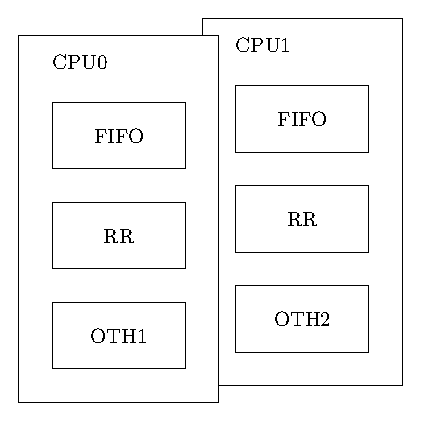
\includegraphics[width=5cm]{proc/objscheds}
  \caption{Scheduler CPU objects for two processor cores and
           per scheduler object scheduling policy objects in
           priority order.}
  \label{figure:objscheds}
\end{figure}
